
\begin{figure*}
\centering
\begin{tabular}{cc}
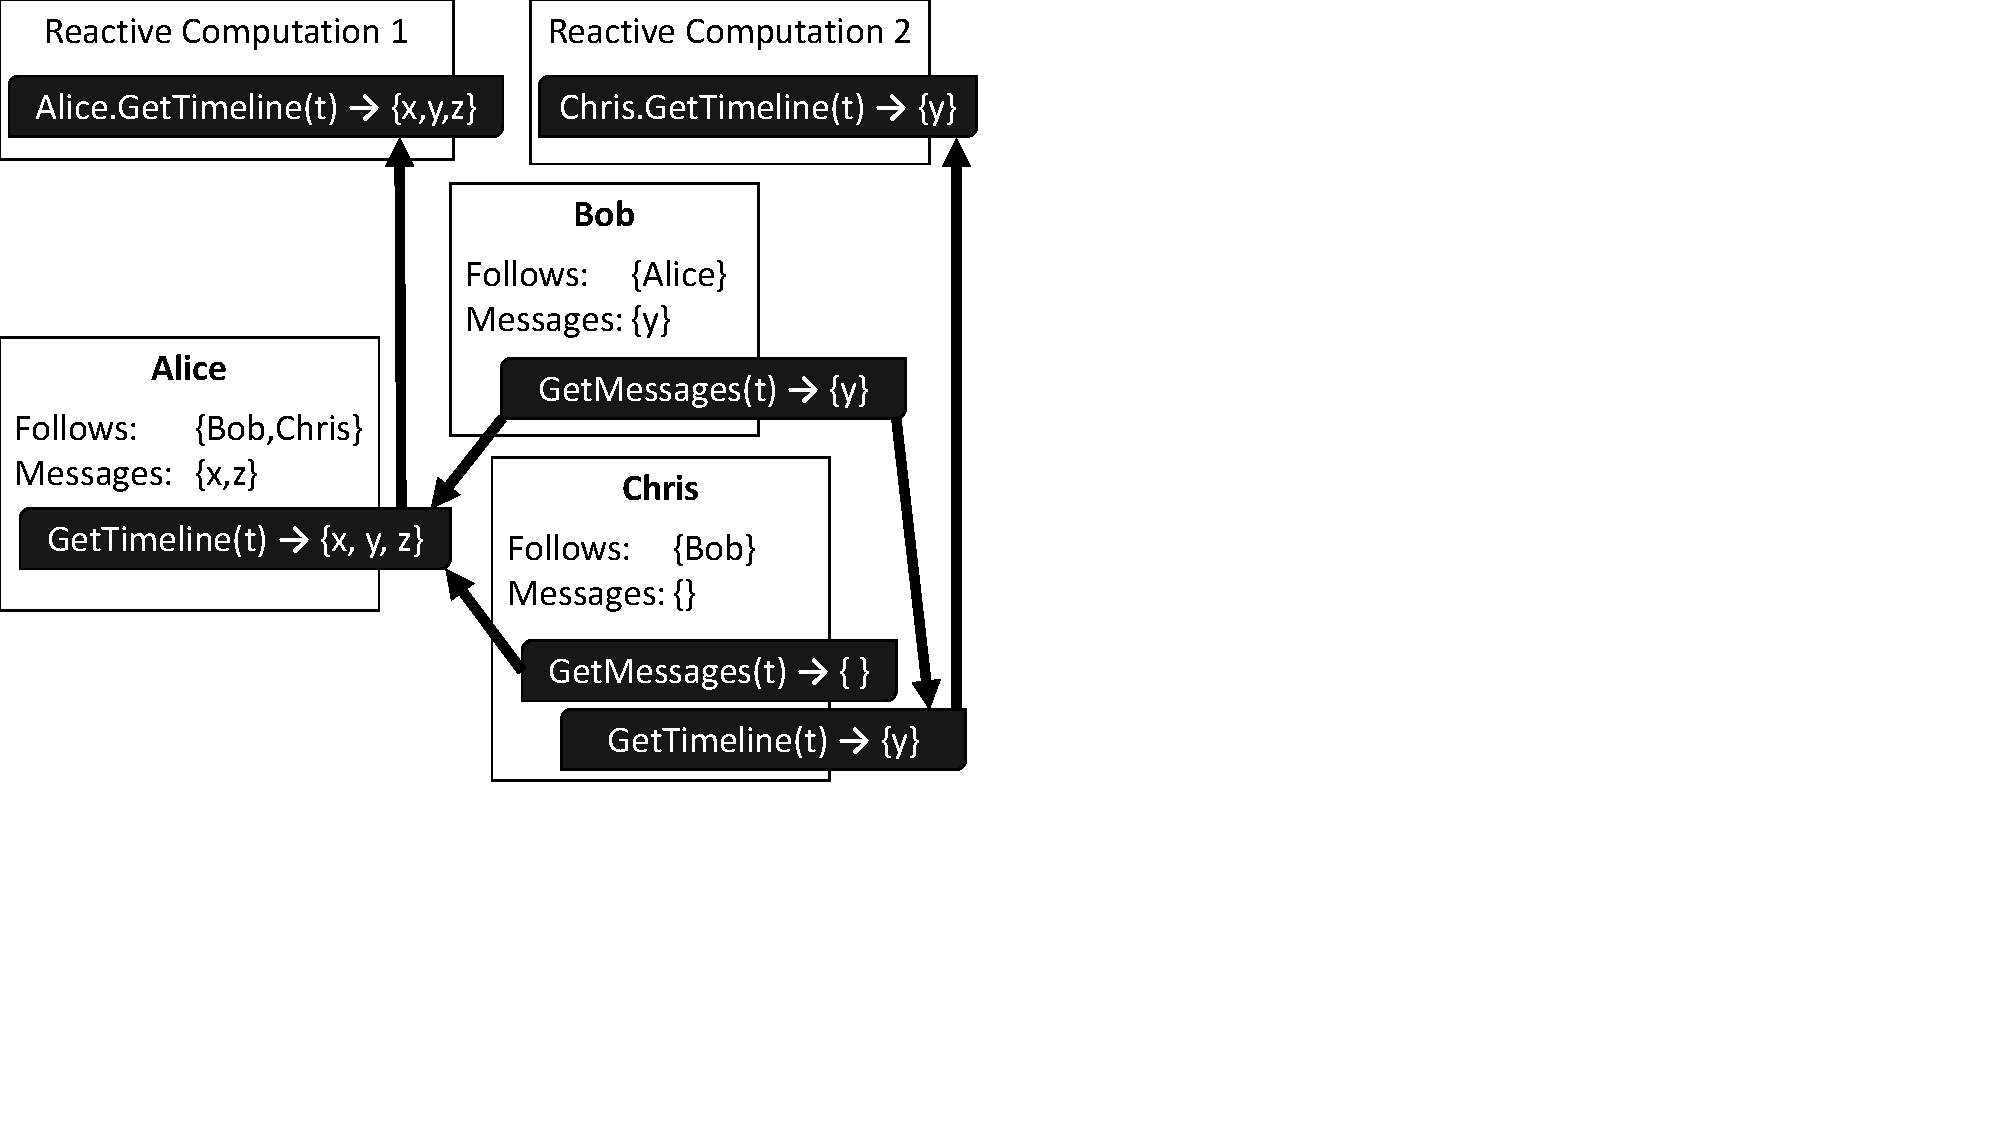
\includegraphics[scale=.45, viewport=-1 164 480 540]{figs/summaries}
&
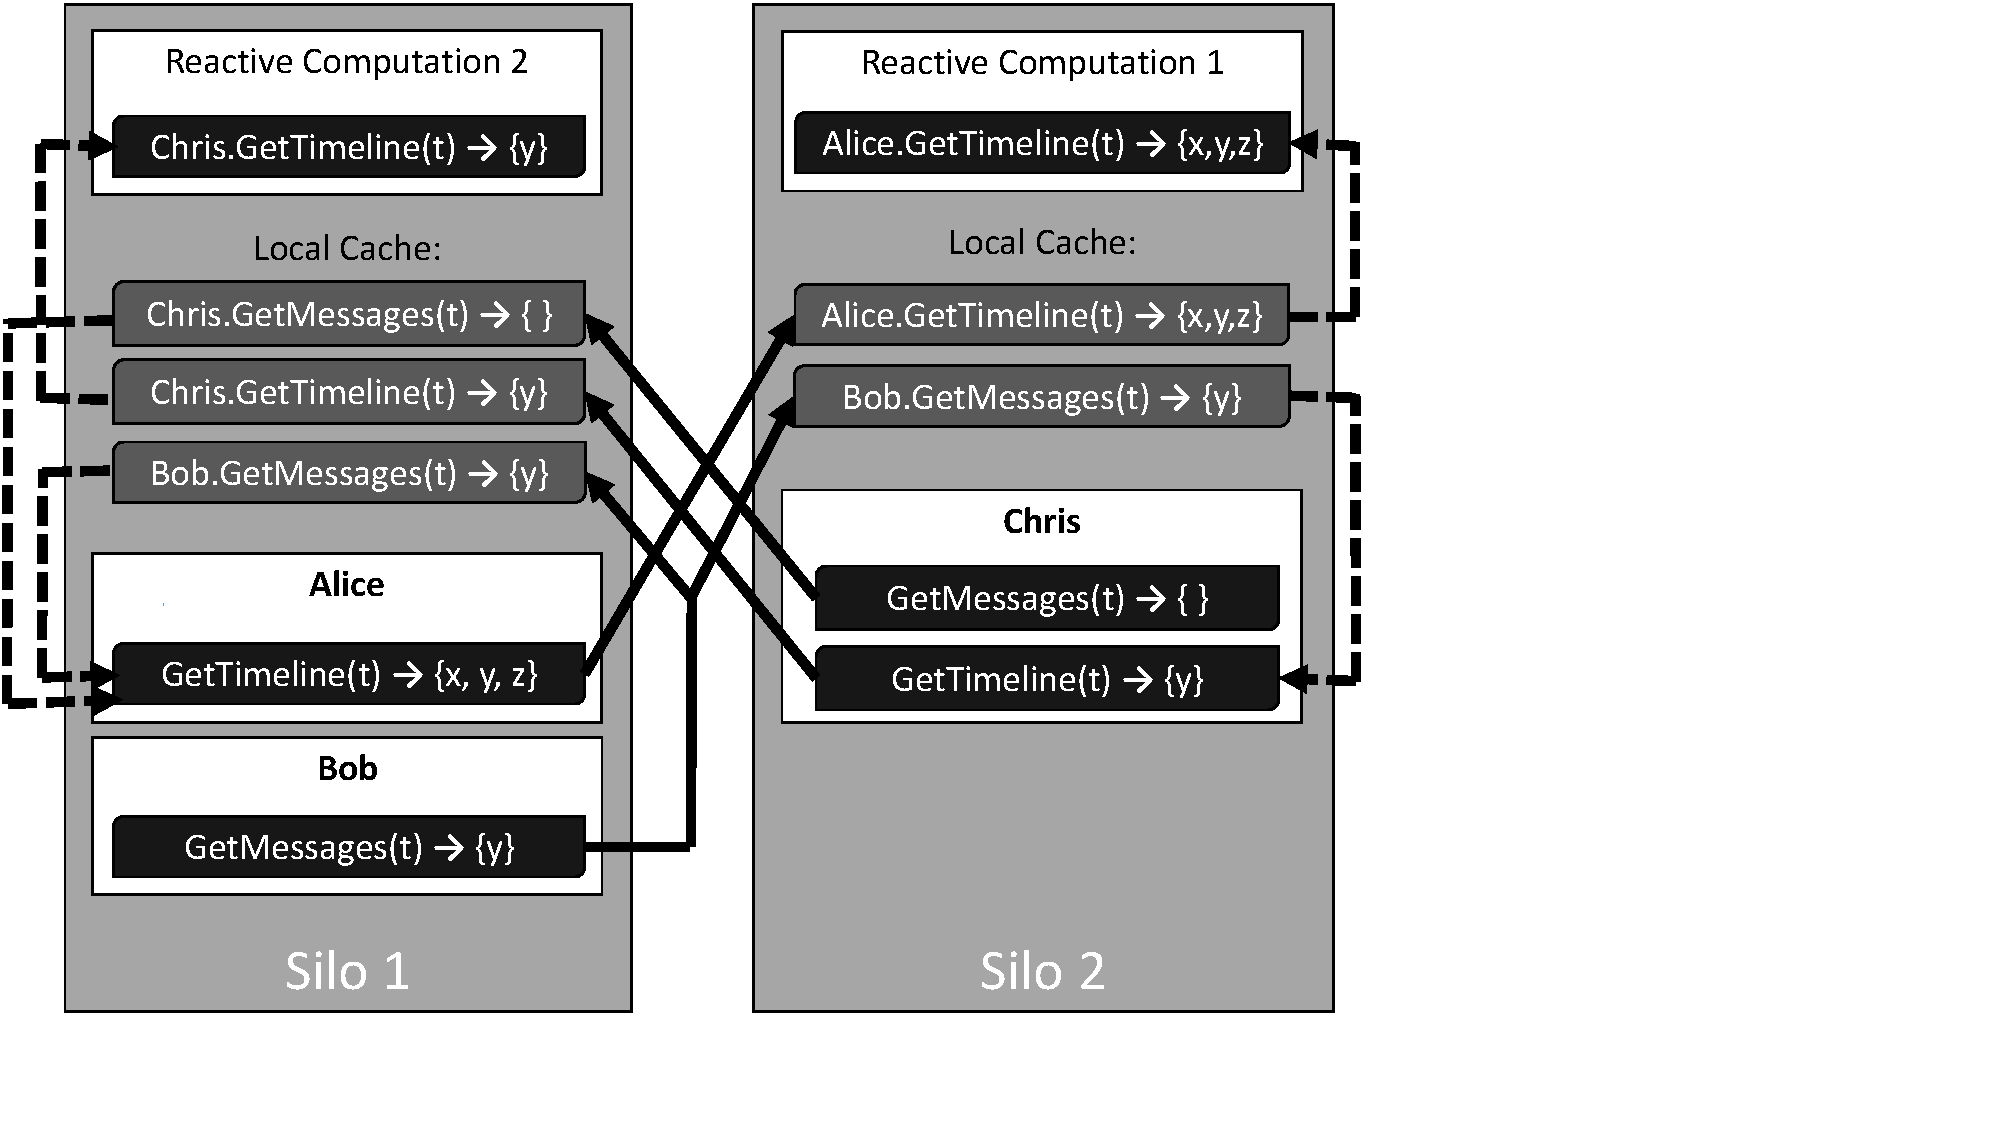
\includegraphics[scale=.4, viewport=-10 53 656 540]{figs/silos}\\
\end{tabular}
\caption{\textbf{(a)}  (on the left) example of a dependency graph of summaries, for two reactive computations; \textbf{(b)} (on the right) example of a corresponding bipartite dependency graph of summaries and local caches, distributed over two silos.}\label{fig:summaries}
\end{figure*}

\section{Reactive Caching Algorithm}\label{sec:algorithm}

To determine when a result of a reactive computation changes, we track all the grains it depends on. Tracking these dependencies is done entirely at runtime and does not require any static analysis: rather, we modify the virtual actor runtime to intercept grain calls and construct a \emph{dependency graph}.

We explain the dependency graph in two stages: first, we describe it as a directed acyclic graph of summaries (\S\ref{sec:summaries}). Then, we show to represent it as a bipartite graph of summaries and caches (\S\ref{sec:bp}) to improve performance and handle failures in a distributed setting. 

\subsection{Summaries and Dependencies}\label{sec:summaries}

During execution, we record and store a \emph{summary} for each executed operation. A summary is a pair consisting of (1) the invoked operation (including grain identity, method name, and all parameters), and (2) the value or exception returned at the end. For each summary, we record what other summaries it depends on, and what summaries depend on it. The result is a \emph{dependency graph} that represents the computation that was performed.

Fig.~\ref{fig:summaries}(a) shows an example of a dependency graph of summaries. Two clients perform reactive computations \lstinline|Alice.GetTimeline(t)| and \lstinline|Chris.GetTimeline(t)| for the same time parameter \lstinline|t|. Summaries are shown as black boxes, and reside either in a grain or in a reactive computation. Summary dependencies are shown as black arrows.

\mypar{Reuse} If a summary for a particular operation already exists, we reuse it. For example, \lstinline|[GetMessages(t)->{y}]| of Bob's grain is shared: two other summaries depend on it. 

\mypar{Re-execution} If a summary is stale (see \S\ref{sec:cp}), it is marked for re-execution. When re-executed, the dependencies may change, and are updated accordingly. 
%After a summary for a reactive computation is re-executed, we push the new result to the client.

\mypar{Garbage Collection} A summary for a grain method is deleted if there are no other summaries that depend on it.  A summary for a reactive computation is deleted when the reactive computation object is disposed. Since the dependency graph is acyclic (a cycle would represent a query with infinite recursion, which is prevented by the runtime), this means that summaries are guaranteed to be collected when no longer needed.  

\subsubsection{Change Propagation}\label{sec:cp}

We call a summary \emph{stale} if a re-execution of the computation or operation would necessarily yield a different result. Our change propagation algorithm guarantees that \emph{any stale summary is eventually re-executed}. Because grains cannot share any state, summaries can become stale for only two reasons: either (1) the state of their grain changes, or (2) a summary they depend on becomes stale.\footnote{We assume that the grain operations used in reactive computations depend only on grain states, and not external state such as clocks or arbitrary I/O.} Thus, the following is sufficient:
\begin{enumerate}
\item Whenever a grain operation changes the state of a grain, we mark all summaries of that grain for re-execution.
\item After a summary for a grain operation is re-executed, we compare the new result to the previous result. If it is the same, no further action is needed. Otherwise, we mark all dependent summaries for re-execution.
\hidden{\item After a summary for a reactive computation is re-executed, we push the new result to the consuming result tracker object.}
\end{enumerate}
 
\noindent For example, executing the operation \lstinline|Chris.Unfollow("Bob")| will mark both of the summaries in Bob's grain for re-execution. Re-execution of \lstinline|[GetMessages(t)->{}]| yields the same result, and propagation stops. But re-execution of \lstinline|[GetTimeline(t)->{y}]| yields a different result \lstinline|{}|, which means we mark the dependent summary in Reactive Computation 2, \lstinline|[Chris.GetTimeline(t)->{y}]|, for re-execution. After it re-executes, the latest result reaches the client as desired.

\paragraph{Ephemeral Inconsistency. }  
%There are no guarantees about the relative consistency of summaries that are used in a computation (since we just use the most recent summary available for a given invocation). 
It is possible for the result of a computation to be inconsistent, in the sense that it is based on versions of grain states that never existed at the same time, or even on different versions of the same grain's state. However, if the result of a computation is inconsistent, then it is also ephemeral: an inconsistent summary must be stale, and is thus guaranteed to be re-executed and replaced.

\mypar{Batching} Some time may pass in between marking a summary for re-execution and the actual re-execution. In particular, it may be marked multiple times, in which case it only needs to be executed once. This batching effect is important for maintaining good throughput under high update frequencies, as we demonstrate in the evaluation section.

\subsection{Reactive Caching}\label{sec:bp}

Under the hood, Orleans' virtual actor runtime load-balances grains across different physical machines called silos. The set of silos can change when administrators choose to increase or decrease the number of servers, or when servers fail (which is detected automatically). By design, the application layer is unaware of the existence of these silos. However, to make our algorithm performant and fault-tolerant, the spatial distribution of grains over silos is relevant, because (1) the latency of a remote call is orders of magnitude higher than the latency of a local call, and (2) silos can fail independently. Thus, we build an extra \emph{caching layer} into the dependency graph.

Rather than summaries that depend directly on other summaries, we now have summaries depend on local caches of summaries. Each summary maintains a connection to all its caches on the various silos, and pushes changes to those caches whenever a re-execution produces a different result. This \emph{reactive caching} mechanism improves performance because it can elide many slow remote accesses in favor of fast lookups in a silo-local hash table.

As an example, consider Fig.~\ref{fig:summaries}(b). It shows a bipartite graph of summaries and caches that corresponds to the dependency graph in Fig.~\ref{fig:summaries}(a). We show two types of edges: summary dependencies (dotted arrows), which are always within a silo, and cache connections (solid lines), which may cross silo boundaries. 

Extending change propagation and garbage collection to the bipartite graph is straightforward: when a cache receives a new value, it marks dependent summaries for re-execution. Caches are removed if they have no summaries that depend on them, and summaries that are not part of a reactive computation are removed if they are not connected to any caches. 

\mypar{Fast Re-execution} When a summary is re-executing, and its dependencies have not changed, all of its grain operations hit in the local cache. Therefore, the overhead of re-execution of summaries is quite low: the latency of our change propagation mechanism is very close to the performance of a hand-written change propagation solution (see \S\ref{sec:evaluation}).

\mypar{Large Fan-out} The reactive caching improves performance in situations with a large fan-out (summaries with many observers): rather than sending updates to each observer directly, it is enough to send one update to each silo, and the silo then forwards the update locally.

\mypar{Back-Pressure} 
Our experiments show that in the case of high update rates, it is beneficial to throttle the sending of updates (only the latest result matters, so intermediate results can be dropped). Our mechanism achieves this by sending results to caches one at a time, and measuring the response time. If above a configurable threshold, we back off (wait for an extra delay equal to the round trip time of the push). 

\subsubsection{Fault Tolerance}

To tolerate faults, we need to make sure that we correctly handle the disappearance of any components that are visible to components on other silos.\footnote{We need not worry about failure of components that are not visible on other silos, because whenever they fail, all components that are aware of them also fail.} In our case, the only thing we need to be concerned about is the connection between summaries and caches (this is readily apparent in Fig.~\ref{fig:summaries}b: the only lines that cross silo boundaries are the solid edges).

Each summary maintains a list of connected caches. To maintain this connection, a cache periodically \emph{re-subscribes} every 30 seconds. This re-subscription allows us to handle one-sided failures as follows:
\begin{itemize}
\item if a cache fails, it will no longer resubscribe. If a summary does not hear from a cache for 90 seconds, it removes it from the list. 
\item if a summary fails, the cache sends a re-subscription after some time --- but the summary, and its associated grain, no longer exist. In that case, the standard virtual actor mechanism re-activates the grain on some silo, and loads its state from persistent storage. Then we recreate the summary and execute it. The cache is now connected to the new instance of the same summary. 
\end{itemize}
